% !TeX root = ../../main.tex
% !TEX spellcheck = en_GB

\section{Design}
\label{ch:Design}
On \cref{fig:DetailedDesign_prepro} is a detailed description of the preprocessing block.
\begin{figure}
	\centering
	\includegraphics[width=1\linewidth]{gfx/Design/DesignDetailed_Preprocesing.pdf}
	\caption{Detailed description of preprocessing in \systemName.}
	\label{fig:DetailedDesign_prepro}
\end{figure}

Input is a time signal, and the output is a discrete signal. Firstly the time signal will be sampled with \SI{48000}{\hertz}. After the signal is sampled it will enter the decimation part, which consist of a lowpass filter with a cutoff at \SI{1200}{\hertz} and stop at \SI{2400}{\hertz}. The downsampling will be a factor $M=10$. The last phase of the proprocessing is too gather the data in a buffer. The buffer size will be 4069, hence the frequency resolution will be $f_{resolution} = \frac{fs_{new}}{size}= \frac{\SI{4800}{\hertz}}{4096}= \SI{1.17}{\hertz}$. An problem with this method is, the time delay that will be created. The closer the size of the buffer gets to $4800$ the closer the delay will become \SI{1}{\second}. An advantage is that the memory usage will be significantly lower then if there was sampled 48000 samples.\newline The output from the preprocessing block will continue too the signal processing block, here a detailed block can be seen on \cref{fig:DetailedDesign_sigpro}.
\begin{figure}
	\centering
	\includegraphics[width=1\linewidth]{gfx/Design/DesignDetailed_Signalprocessing.pdf}
	\caption{Detailed description of signal processing in \systemName.}
	\label{fig:DetailedDesign_sigpro}
\end{figure}

Input to the signal processing block is the discrete signal which was the output from the preprocessing block. The output from signal processing is, the new changed discrete signal where the frequency has been changed. The input signal will go too the FFT block, here $fs=\SI{4800}{\hertz}$ and $n=4096$. The FFT block will have as output the transformed signal called xfft. xfft will be passed onto the block FindMax which will find the max frequency and the corresponding bin nr. FindMax will then pass on this information to the PitchShift Algorithm which will use this information on the discrete input signal. As output will the new discrete signal with a new frequency. The challenge is the end of each processed block has to match the next block of data. Therefore a future extension would be to make each block overlap so they match eachother. The output from signal processing will be passed on to the postprocessing block which can be seen on \cref{fig:DetailedDesign_postpro}. 

\begin{figure}
	\centering
	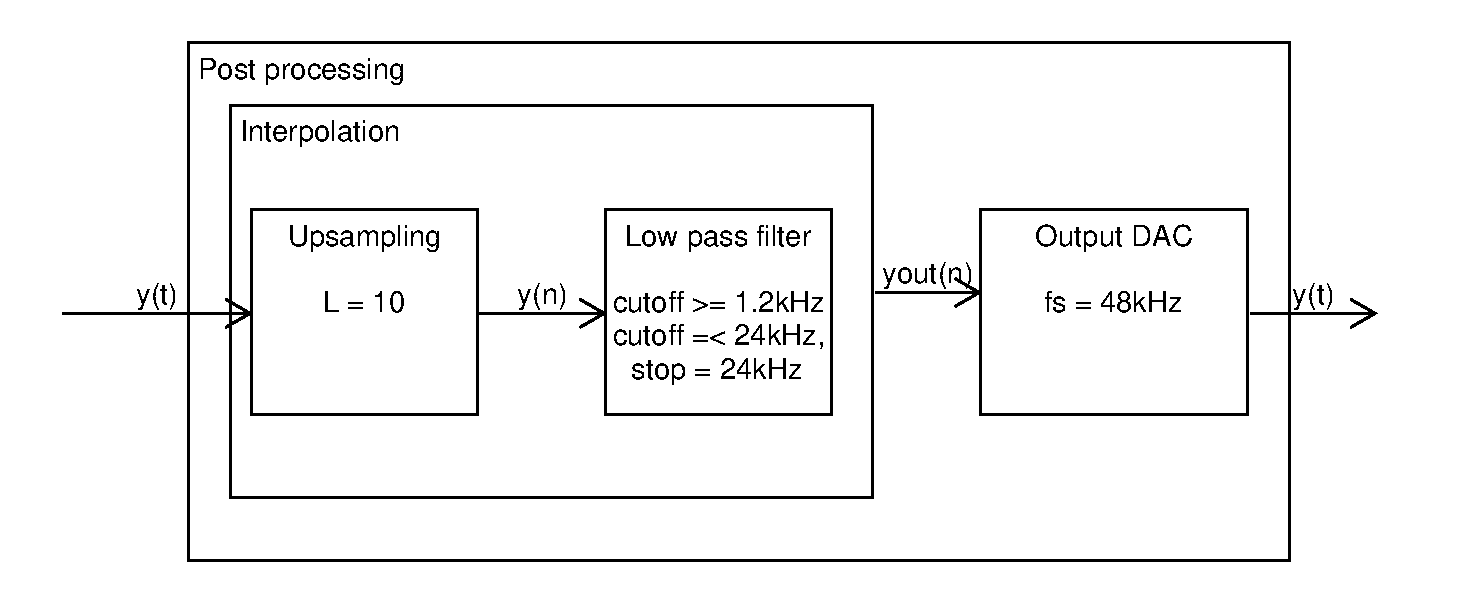
\includegraphics[width=1\linewidth]{gfx/Design/DesignDetailed_Postprocessing.pdf}
	\caption{Detailed description of postprocessing in \systemName.}
	\label{fig:DetailedDesign_postpro}
\end{figure}

The main function of the post processing block is to upsample the signal so it can be played send out by the DAC at a $fs=\SI{48000}{\hertz}$. The interpolation is an integer of 10, followed up by a lowpass filter. The DAC will send out the final signal which shoulde have a new frequency now compared to the input signal. \fxnote{Move this to an appendix}


\FloatBarrier